This section specifies the software architecture requirements and the software
architecture design for web application framework.

\subsection{Architecture Requirements}
The web application framework provides the software architecture for the software
providing browser based access to human users.

\subsubsection{Access and Integration Requirements}
\paragraph*{Access Channel Requirements}
The web application framework will address the human access channel requirement
referred to in section \ref{sec:humanAccessChannelManagementSystem}. As this 
implementation of the system is a prototype, we will only be supporting the
latest Google Chrome web browser. The web application is however HTML5 compliant.

\paragraph*{Integration Channel Requirements}
The web application must integrate with the management system in order to allow
users to derive value. However, the web application will integrate with the
business layer through the web services layer, allowing one to decouple the
business and presentation layers from one another.

\subsubsection{Quality Requirements}
\paragraph*{Usability}
It is important that users using the system feel as though the system delivers
what they require, when they require it.

\paragraph*{Maintainability}
The system as a whole should be easily expandable, for this reason a modern
JavaScript framework such as Angular2 was chosen to assist developers
to maintain the system much easier, allowing the code base to mature
with time without losing strict control and structure.



\subsection{Architecture Design}
This section specifies the software architecture design for a third level granularity com-
ponent, namely the web interface. The architecture design include the allocation of
architectural responsibilities to architectural components, as well as tactics used to real-
ize these responsibilities under the current level of granularity to address stated quality
requirements.



\subsection{Architectural Responsibilities, Components and Realization}
The architectural components of the  Web Application Framework are shown in Figure \ref{fig:webApplicationFrameworkResponsibilityAllocation}
\begin{figure}[H]
	\begin{center}
	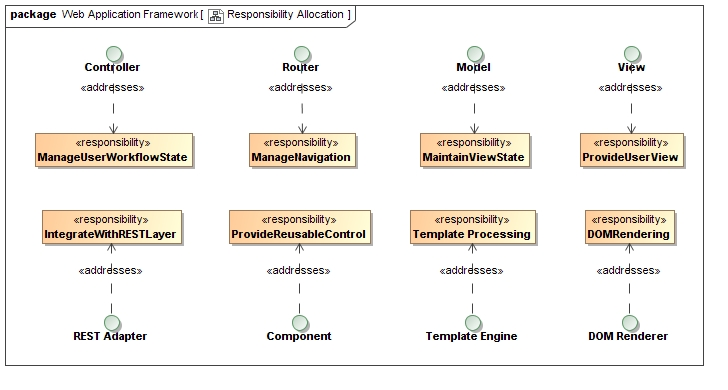
\includegraphics[scale=0.5]{../Diagrams and Charts/Web Application Framework/Responsibility Allocation.jpg}
	\caption{The abstract components to which the Web Application Framework responsibilities are assigned.}
	\label{fig:webApplicationFrameworkResponsibilityAllocation}
	\end{center}
\end{figure}



\subsubsection{Tactics}
Tactics Angular2 uses in order to address the quality requirements should include:
\begin{itemize}
	\item caching of pre-generated and pre-populated HTML pages for performance
	\item virtual DOM for in-memory updates, incremental builds and efficient 
	diffing based on differentiation between static and dynamic DOM elements
\end{itemize}



\subsubsection{Frameworks and Technologies}
The web framework the project will be utilizing will be based on Angular2
which is a JavaScript framework developed by Google Inc. Angular2 is an 
open-source web application framework which promises a one-way flow of 
information between  model, controller and view. This promise is meant to 
increase performance and decoupling of the underlying code thereby assisting
with maintainability.

Core reasons for using Angular2 include:
\begin{itemize}
	\item Framework requires a defined structure which aids in maintainability.
	\item The framework is maintained not only by a community of users but also
	by Google, which aids in maintainability due to the 
	constant upkeep of the code base and documentation.
	\item Angular2 supports very good integration with RESTful API services.
\end{itemize}

Other frameworks that were considered;
\begin{itemize}
	\item ReactJS
	\item Ember.js 
	\item Backbone.js
\end{itemize}
